\chapter{INTRODUCTION}
\label{chap:introduction}

Call acronym: \ac{DoF}, \ac{FRVF}.

\lipsum[1-2]

\chapter{OBJECTIVE}
\label{chap:objetive}

On line citation \citeonline{earnshaw2014virtual}.
Normal cite: \cite{earnshaw2014virtual}. Multiple citation: \cite{azuma1997survey, earnshaw2014virtual}.

\section{Topic a}

\lipsum[1]

In Table~\ref{tab:autonomy} ...

\begin{table}[htb]
	\centering
	\caption{Flight autonomy.}
	\label{tab:autonomy}
	\begin{tabular}{l|l|l|}
		\cline{2-3} & Towers 51-50 & Towers 49-50 \\ \hline
		\multicolumn{1}{|l|}{Flight time}         & 11m54s       & 09m14s       \\ \hline
		\multicolumn{1}{|l|}{Battery on takeoff} & 74\%         & 80\%         \\ \hline
		\multicolumn{1}{|l|}{Battery on landing}     & 33\%         & 48\%         \\ \hline
		\multicolumn{1}{|l|}{Max speed}    & 12,5 km/h    & 21,3 km/h    \\ \hline
	\end{tabular}
	\legend{Source: The authors.}
\end{table}

\section{Topic b}

\lipsum[1]

\chapter{EXPERIMENTAL PROCEDURE} 
\label{chap:methodology}

It should contain the description of the study area and materials (data bank, data collection, images, etc.) and methodological procedures (experiments, interviews, statistical methods, etc.) that will be used to carry out the work, so that others researchers can reproduce the study. It can be presented as subdivisions below.

\begin{itemize}
	\item \textbf{AHA}: \large \textit{The American Heart Association Database for Evaluation of Ventricular Arrhythmia Detectors}.
	\item \textbf{MIT–BIH}: \large \textit{The Massachusetts Institute of Technology–Beth Israel Hospital Arrhythmia Database}.
	\item \textbf{ESC}: \large \textit{The European Society of Cardiology ST-T Database} (90 records of 2 hours each).
	\item \textbf{NST}: \large \textit{The Noise Stress Test Database}.
	\item \textbf{CU}: \large \textit{The Creighton University Sustained Ventricular Arrhythmia Database}.
\end{itemize}

\section{MIT-BIH}

\begin{figure}[htb]
	\caption{Beat examples.}
	\begin{center}  
		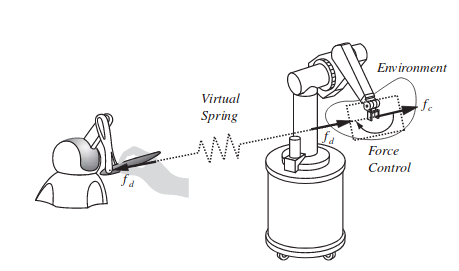
\includegraphics[scale=0.6]{img/examples/haptic.png}
	\end{center}
	\legend{Source: \cite[p. 13]{earnshaw2014virtual}}
	\label{fig_mitbih}
\end{figure}

\subsection{Sub section}

\begin{table}[htb]
	\centering
	\caption{Records used and number of representatives of each class for each of the partitions.}
	\begin{adjustbox}{width=1\textwidth}
		\label{tabela-particoes}
		\begin{tabular}{|c|c|c|c|c|c|c|}
			\hline
			\rowcolor[HTML]{D0D0D0}
			Partition                     & Registry                                                                                                                                              & Class N & Class SVEB & Class VEB \\ \hline
			\hline      
			\cellcolor[HTML]{EFEFEF}DS1   & 101, 106, 108, 109, 112, 114, 115, 116, 118, 119, 122, 124, 201, 203, 205, 207, 208, 209, 215, 220, 223, 230 & 45543    & 782         & 3469       \\ \hline        
			\cellcolor[HTML]{EFEFEF}DS11  & 101, 106, 108, 109, 114, 115, 116, 119, 122, 209, 223                                                                                                  & 22249    & 474         & 1615       \\ \hline      
			\cellcolor[HTML]{EFEFEF}DS12  & 112, 118, 124, 201, 203, 205, 207, 208, 215, 220, 230                                                                                                  & 23294    & 308         & 1854       \\ \hline  
			\cellcolor[HTML]{EFEFEF}DS2   & 100, 103, 105, 11, 113, 117, 121, 123, 200, 202, 210, 212, 213, 214, 219, 221, 222, 228, 231, 232, 233, 234  & 44049    & 1808        & 3143       \\ \hline
			\rowcolor[HTML]{B8B8B8} 
			\cellcolor[HTML]{EFEFEF}Total &                                                                                                                                                        & 89592    & 2590        & 6612       \\ \hline
		\end{tabular}
	\end{adjustbox}
	\legend{Source: The authors.}
	\label{table:aa}
\end{table}

\subsubsection{Sub sub section}

Equation example:

\begin{equation}
w_{ij} = e_{i,j} = \sqrt{(x_i - x_j)^2 + (y_i - y_j)^2 + (z_i - z_j)^2},
\label{eq:edge}
\end{equation}

\begin{algorithm}
	\caption{Euclid’s algorithm}\label{alg:euclid}
	\begin{algorithmic}[1]
		\Procedure{Euclid}{$a,b$}\Comment{The g.c.d. of a and b}
		\State $r\gets a\bmod b$
		\While{$r\not=0$}\Comment{We have the answer if r is 0}
		\State $a\gets b$
		\State $b\gets r$
		\State $r\gets a\bmod b$
		\EndWhile\label{euclidendwhile}
		\State \textbf{return} $b$\Comment{The gcd is b}
		\EndProcedure
	\end{algorithmic}
\end{algorithm}

\begin{equation}
\label{eq:sigmoide}
s(v)=\frac{1}{1+\exp(-v)}
\end{equation}

\begin{figure}[htb]
	\begin{center} 
		\caption{Behavior of the sigmoid function for values between -10 and 10.} 
		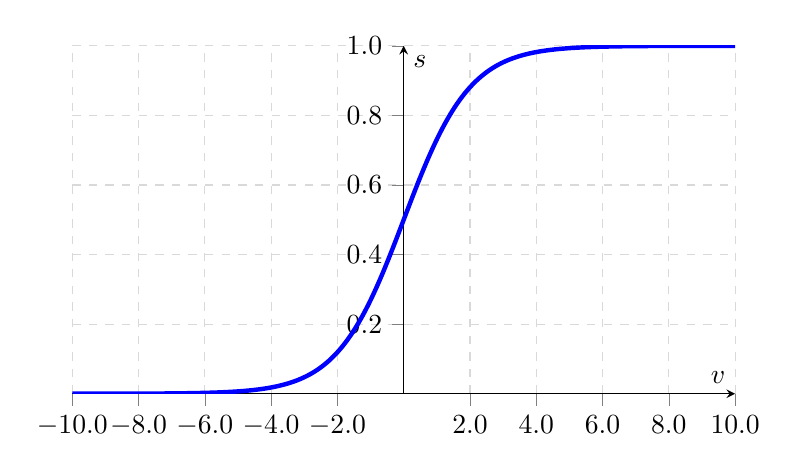
\begin{tikzpicture}
		\begin{axis}[
		legend pos=north west,
		axis x line=middle,
		axis y line=middle,
		x tick label style={/pgf/number format/fixed,
			/pgf/number format/fixed zerofill,
			/pgf/number format/precision=1},
		y tick label style={/pgf/number format/fixed,
			/pgf/number format/fixed zerofill,
			/pgf/number format/precision=1},
		grid = major,
		width=10cm,
		height=6cm,
		grid style={dashed, gray!30},
		xmin=-10,     % start the diagram at this x-coordinate
		xmax= 10,    % end   the diagram at this x-coordinate
		ymin= 0,     % start the diagram at this y-coordinate
		ymax= 1,   % end   the diagram at this y-coordinate
		%axis background/.style={fill=white},
		xlabel=$v$,
		ylabel=$s$,
		tick align=outside,
		enlargelimits=false]
		% plot the stirling-formulae
		\addplot[domain=-10:10, blue, ultra thick,samples=500] {1/(1+exp(-x))};
		\end{axis}
		\end{tikzpicture}
	\end{center}
	\legend{Source: The authors.}
	\label{fig_sigmoide}
\end{figure}

\chapter{RESULTS}

\lipsum[1-2]

\chapter{DISCUSSION}

To present the discussions of the results obtained in the present study with those of previous publications, highlighting their contribution on the subject.

\chapter{CONCLUSION}

Mention the main conclusions of the dissertation highlighting the points mentioned in the specific objectives.

\chapter{RECOMMENDATIONS}

Mention the possible developments of the research and the suggestions for the continuation of the work.